% !TEX root = ../AnonymousSubmission2027.tex
\section{Introduction}
\label{sec:intro}

\begin{figure}[t]
    \centering
    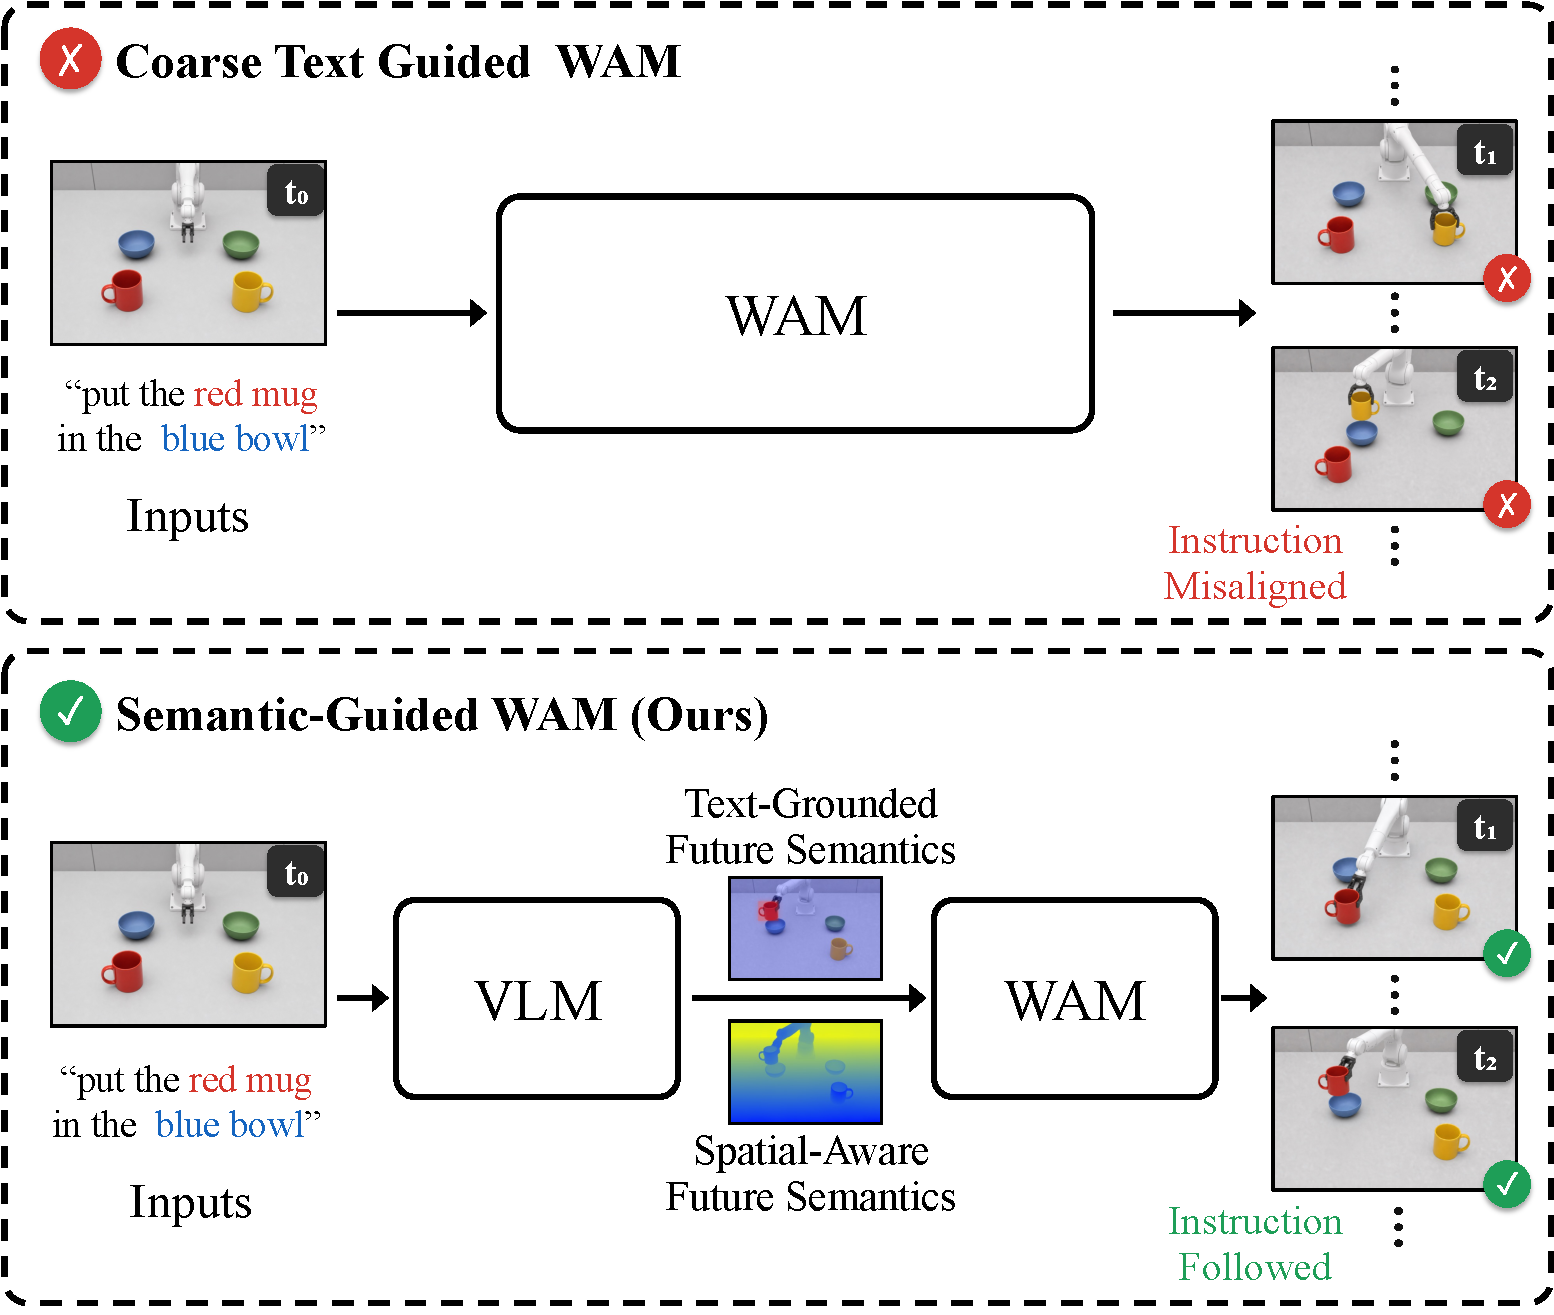
\includegraphics[width=\columnwidth]{Figures/teaser-v0.pdf}
    \caption{Our method introduces a VLM semantic planner that predicts text-grounded and spatial-aware semantic foresight of the intended future and uses it to guide the world-action model, so that both the generated videos and actions faithfully follow the language instruction.}
    \label{fig:teaser}
\end{figure}

\IEEEPARstart{W}{orld-Action} Models (WAMs) have recently emerged as a promising paradigm for robotic manipulation~\cite{uwm,worldvla,dit4dit,maskwam,dswam}.
Instead of mapping observations and instructions directly to actions as in vision-language-action (VLA) policies~\cite{brohan2023rt,zitkovich2023rt,kim2024openvla,BlackK-RSS-25}, WAMs learn physical dynamics and task-relevant temporal structure by jointly predicting future observations and actions.
This predictive formulation leads to strong performance and generalization across a wide range of manipulation tasks, and further allows WAMs to be pretrained on large-scale video data in addition to robot demonstrations~\cite{unipi,gr1}.

Despite this progress, most existing video-based WAMs~\cite{vpp,lingbotva,genieenvisioner,fastwam} generate future frames and actions by relying mainly on visual cues rather than on the language instruction. 
The instruction enters generation only through text embeddings from off-the-shelf text encoders such as CLIP and T5~\cite{radford2021learning,raffel2020exploring}, computed independently of the visual observation.
The action expert therefore relies on dynamic features that are poorly aligned with the instruction~\cite{liberoplus}. This poor alignment directly degrades manipulation performance.

To overcome this limitation, there have been efforts to use explicit spatial cues for world-action models~\cite{maskwam,maskwm}, but such cues still fall short of fine-grained and instruction-level semantics.
In this paper, we propose \ourmethod, a semantic guidance paradigm for world-action models (see Figure~\ref{fig:teaser}). Within this paradigm, world-action models are guided by text-grounded and spatial-aware semantic foresight instead of observation-independent text embeddings: the text-grounded semantics ground the instruction in the scene so that the model acts on the correct target objects, while the spatial-aware semantics supply the scene geometry needed to manipulate them precisely.
\rev{Throughout this paper, ``text-grounded'' has a specific operational meaning: the foresight is supervised in a language-aligned visual feature space, namely the SigLIP2~\cite{siglip2} features of future frames, which are themselves extracted from images alone, and the instruction enters through the planner input, so that the instruction determines which future is predicted in that space. It does not denote explicit grounding of individual phrases to image regions.}
Together, they offer a fine-grained and structured blueprint for both future video and action prediction.

Specifically, as shown in Figure~\ref{fig:overview}, our \ourmethod consists of two components: a VLM planner that predicts the semantic guidance, and a world-action model that generates the future video and actions under this guidance.
We implement the planner by appending learnable query tokens to the image--instruction sequence and decoding the foresight from their hidden states in a single forward pass.
The tokens consist of a base group and two modality-specific groups: the base group learns the shared semantic knowledge, while the two specific groups learn text-grounded and spatial-aware semantics, respectively.
For the text-grounded semantic guidance, we align its output representations with the future-frame features of a language-aligned foundation model~\cite{siglip2}, which grounds the predicted semantics in the language instruction.
For the spatial-aware semantic guidance, we align its representations with those of a geometry foundation model~\cite{lin2025depth}, which provides the scene geometry required for precise manipulation.
The semantic foresight serves as a high-level blueprint that conditions the video expert, steering future prediction toward the intended semantics while preserving the pretrained generative ability of the video expert.
The action expert then decodes actions from this foresight-conditioned video expert, so that the predicted video and the executed actions stay consistent with the language instruction.

We comprehensively evaluate \ourmethod across both simulation benchmarks and a physical dual-arm robotic system.
Experiments on the LIBERO~\cite{liu2023libero} and LIBERO-Plus~\cite{liberoplus} benchmarks demonstrate that our method achieves state-of-the-art (SOTA) performance and remains robust under environmental and instruction perturbations.
Furthermore, we deploy \ourmethod as a closed-loop controller on an AgileX Cobot platform with two 6-DoF arms and three RGB cameras, where the predicted joint-space action chunks are executed in a receding-horizon manner and tracked by the low-level joint controllers.
These hardware experiments confirm that our model transfers its instruction-following and precise-manipulation capabilities to physical environments, including container heights and lighting conditions never seen during data collection.
In summary, our contributions are:
\begin{itemize}
    \item We propose a new semantic-guided prediction paradigm for world-action models, guiding both future and action prediction with text-grounded and spatial-aware semantic foresight rather than observation-independent text embeddings.

    \item We introduce \ourmethod, an instantiation of this paradigm built on a VLM planner that predicts complementary text-grounded and spatial-aware semantic foresight, enabling both future video and action generation to faithfully follow the language instruction.

    \item We integrate \ourmethod into a closed-loop control pipeline on a physical dual-arm platform. Extensive experiments in simulation and on this hardware show that \ourmethod achieves state-of-the-art performance, delivering precise manipulation and strong instruction following.
\end{itemize}
